
\documentclass[11pt]{article}
\usepackage[a4paper,margin=1in]{geometry}
\usepackage{amsmath,amssymb}
\usepackage{graphicx}
\usepackage[dvipsnames]{xcolor}
\usepackage{hyperref}
\usepackage{enumitem}
\usepackage{tabularx}
\usepackage{longtable}
\usepackage{booktabs}
\usepackage[most]{tcolorbox}
\usepackage{titlesec}
\usepackage{xurl}
\usepackage{fancyhdr}
\usepackage{setspace}
\usepackage{tikz}
\usetikzlibrary{positioning,arrows.meta}
\usepackage[T1]{fontenc}
\usepackage{lmodern}
\setlength{\parindent}{0pt}
\setlength{\parskip}{8pt}
\setlength{\headheight}{14pt}
\setstretch{1.12}
\setlist[itemize]{leftmargin=1.5em, nosep}
\setlist[enumerate]{leftmargin=1.5em, nosep}
\providecommand{\tightlist}{\setlength{\itemsep}{0pt}\setlength{\parskip}{0pt}}
\hypersetup{colorlinks=true,linkcolor=MidnightBlue,urlcolor=MidnightBlue}
\pagestyle{fancy}
\fancyhf{}
\rhead{\thepage}
\renewcommand{\headrulewidth}{0pt}
\renewcommand{\footrulewidth}{0pt}
\titleformat{\section}{\Large\bfseries\color{MidnightBlue}}{\thesection}{0.6em}{}
\titleformat{\subsection}{\bfseries}{}{0em}{}


\begin{document}

\begin{center}\LARGE\bfseries DDN and POMDP Synthesis\end{center}

\begin{center}\large Block 4 Day 5\end{center}

\begin{tcolorbox}[colback=MidnightBlue!4,colframe=MidnightBlue,title={Session Overview},fonttitle=\bfseries,breakable]
\textbf{Session objective:} Synthesize temporal belief, decision structure, and partially observed planning across healthcare and other applied domains.

\textbf{Timing target (min):} 72

\textbf{Topic anchors:} dynamic bayesian network; dynamic decision network; partially observable markov decision process; healthcare; belief update; human-in-the-loop

\textbf{Padlet board:} \url{https://padlet.com/qmul/b4-d5-2xwxr9vzgkizrx5z}
\end{tcolorbox}

\section*{Exercises}

\begin{tcolorbox}[colback=white,colframe=MidnightBlue,title={Q1 Core Concept Check},fonttitle=\bfseries,breakable]
\begin{center}
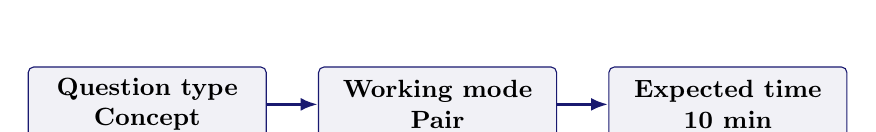
\begin{tikzpicture}[
node distance=0.65cm,
box/.style={draw=MidnightBlue, rounded corners=2pt, minimum height=0.95cm, align=center, font=\small\bfseries, fill=MidnightBlue!6, text width=0.23\linewidth},
arrow/.style={-{Latex[length=2.2mm]}, very thick, MidnightBlue}
]
\node[box] (type) {Question type\\Concept};
\node[box, right=of type] (mode) {Working mode\\Pair};
\node[box, right=of mode] (time) {Expected time\\10 min};
\draw[arrow] (type) -- (mode);
\draw[arrow] (mode) -- (time);
\end{tikzpicture}
\end{center}

{\large\bfseries\color{MidnightBlue} Prompt}\par\medskip
In a healthcare decision-support pipeline, what distinct job would you give to a dynamic Bayesian network (DBN), a dynamic decision network (DDN), and a partially observable Markov decision process (POMDP)? Add one sentence explaining how the three pieces connect.

{\large\bfseries\color{MidnightBlue} Task details}\par\medskip
\begin{itemize}\item \textbf{Type:} concept
\item \textbf{Mode:} pair
\item \textbf{Time:} 10 min
\item \textbf{Deliverable:} model-role mapping
\item \textbf{Assessment focus:} map the roles of dynamic Bayesian networks, dynamic decision networks, and partially observable Markov decision processes
\item \textbf{Expected length:} 3 rows + 1 link sentence\end{itemize}

{\large\bfseries\color{MidnightBlue} How to submit}\par\medskip
Post one pair Padlet comment as a three-row table plus one linking sentence.

{\large\bfseries\color{MidnightBlue} Discussion in class}\par\medskip
Which model is hardest to replace with a simpler one?

{\large\bfseries\color{MidnightBlue} Why this helps}\par\medskip
Useful for synthesis questions that separate temporal state estimation, decision structure, and partial observability.

{\large\bfseries\color{MidnightBlue} References}\par\medskip
\begin{itemize}\item Russell \& Norvig (2021) AIMA 4e, Ch.17-18
\item Poole \& Mackworth (2023) 3e, Ch.12-13, pp.517-608\end{itemize}
\end{tcolorbox}

\begin{tcolorbox}[colback=white,colframe=MidnightBlue,title={Q2 Structured Problem},fonttitle=\bfseries,breakable]
\begin{center}
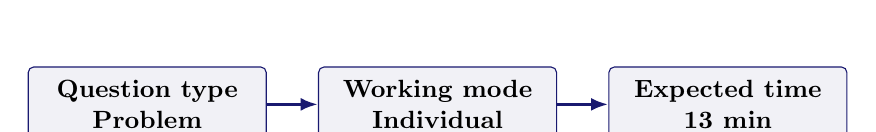
\begin{tikzpicture}[
node distance=0.65cm,
box/.style={draw=MidnightBlue, rounded corners=2pt, minimum height=0.95cm, align=center, font=\small\bfseries, fill=MidnightBlue!6, text width=0.23\linewidth},
arrow/.style={-{Latex[length=2.2mm]}, very thick, MidnightBlue}
]
\node[box] (type) {Question type\\Problem};
\node[box, right=of type] (mode) {Working mode\\Individual};
\node[box, right=of mode] (time) {Expected time\\13 min};
\draw[arrow] (type) -- (mode);
\draw[arrow] (mode) -- (time);
\end{tikzpicture}
\end{center}

{\large\bfseries\color{MidnightBlue} Prompt}\par\medskip
A patient has prior high-risk belief 0.25 at time t. The transition model is P(High\_t+1\textbar High\_t)=0.70 and P(High\_t+1\textbar Low\_t)=0.15. The observation model is P(Alert+\textbar High)=0.80 and P(Alert+\textbar Low)=0.30. After observing Alert+, compute the posterior belief that the patient is high risk at time t+1.

\begin{tcolorbox}[colback=ForestGreen!5,colframe=ForestGreen,title={Formula reminder},fonttitle=\bfseries,breakable]
\[
b'(s')=\alpha \, P(o \mid s') \sum_{s} P(s' \mid s,a)\,b(s)
\]
\textbf{Use this when the task asks for a filtered or belief-state update.}
\end{tcolorbox}

{\large\bfseries\color{MidnightBlue} Task details}\par\medskip
\begin{itemize}\item \textbf{Type:} problem
\item \textbf{Mode:} individual
\item \textbf{Time:} 13 min
\item \textbf{Deliverable:} belief update computation
\item \textbf{Assessment focus:} compute a prediction step and posterior belief after a noisy observation
\item \textbf{Expected length:} 5 calculation lines\end{itemize}

{\large\bfseries\color{MidnightBlue} How to submit}\par\medskip
Post your own Padlet comment showing the prediction step, the evidence update, the normalization step, and the final posterior.

{\large\bfseries\color{MidnightBlue} Discussion in class}\par\medskip
Why does the positive alert increase belief without making the patient certainly high risk?

{\large\bfseries\color{MidnightBlue} Why this helps}\par\medskip
Direct practice for belief-state updates while using different numbers from the exam-style examples.

{\large\bfseries\color{MidnightBlue} References}\par\medskip
\begin{itemize}\item Russell \& Norvig (2021) AIMA 4e, Ch.17-18
\item Poole \& Mackworth (2023) 3e, Ch.12-13, pp.517-608\end{itemize}
\end{tcolorbox}

\begin{tcolorbox}[colback=white,colframe=MidnightBlue,title={Q3 Structured Problem},fonttitle=\bfseries,breakable]
\begin{center}
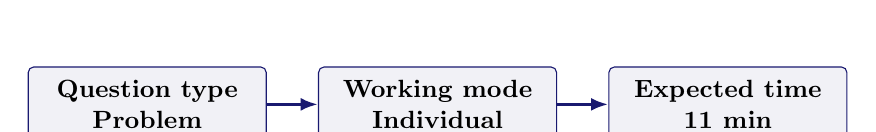
\begin{tikzpicture}[
node distance=0.65cm,
box/.style={draw=MidnightBlue, rounded corners=2pt, minimum height=0.95cm, align=center, font=\small\bfseries, fill=MidnightBlue!6, text width=0.23\linewidth},
arrow/.style={-{Latex[length=2.2mm]}, very thick, MidnightBlue}
]
\node[box] (type) {Question type\\Problem};
\node[box, right=of type] (mode) {Working mode\\Individual};
\node[box, right=of mode] (time) {Expected time\\11 min};
\draw[arrow] (type) -- (mode);
\draw[arrow] (mode) -- (time);
\end{tikzpicture}
\end{center}

{\large\bfseries\color{MidnightBlue} Prompt}\par\medskip
Give two similarities and two differences between a dynamic decision network and a POMDP. Keep the answer in simple language and focus on what each model makes easier to express.

{\large\bfseries\color{MidnightBlue} Task details}\par\medskip
\begin{itemize}\item \textbf{Type:} problem
\item \textbf{Mode:} individual
\item \textbf{Time:} 11 min
\item \textbf{Deliverable:} model comparison note
\item \textbf{Assessment focus:} compare dynamic decision networks and POMDPs without treating them as synonyms
\item \textbf{Expected length:} 4 bullets\end{itemize}

{\large\bfseries\color{MidnightBlue} How to submit}\par\medskip
Post your own Padlet comment as four bullets.

{\large\bfseries\color{MidnightBlue} Discussion in class}\par\medskip
Which model makes the role of belief state more explicit?

{\large\bfseries\color{MidnightBlue} Why this helps}\par\medskip
Useful for comparison questions that test conceptual understanding rather than only notation.

{\large\bfseries\color{MidnightBlue} References}\par\medskip
\begin{itemize}\item Russell \& Norvig (2021) AIMA 4e, Ch.17-18
\item Poole \& Mackworth (2023) 3e, Ch.12-13, pp.517-608\end{itemize}
\end{tcolorbox}

\begin{tcolorbox}[colback=white,colframe=MidnightBlue,title={Q4 Collaborative Mini-Case},fonttitle=\bfseries,breakable]
\begin{center}
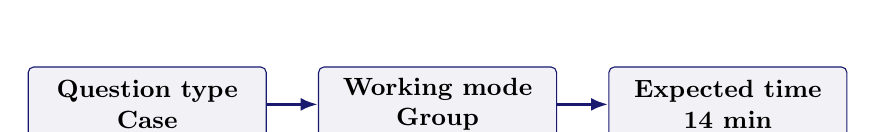
\begin{tikzpicture}[
node distance=0.65cm,
box/.style={draw=MidnightBlue, rounded corners=2pt, minimum height=0.95cm, align=center, font=\small\bfseries, fill=MidnightBlue!6, text width=0.23\linewidth},
arrow/.style={-{Latex[length=2.2mm]}, very thick, MidnightBlue}
]
\node[box] (type) {Question type\\Case};
\node[box, right=of type] (mode) {Working mode\\Group};
\node[box, right=of mode] (time) {Expected time\\14 min};
\draw[arrow] (type) -- (mode);
\draw[arrow] (mode) -- (time);
\end{tikzpicture}
\end{center}

{\large\bfseries\color{MidnightBlue} Prompt}\par\medskip
Design an end-to-end healthcare decision-support workflow using a data agent, a state-estimation agent, a policy agent, and a safety or human-oversight gate. Include the points where evidence, belief, recommendation, and approval appear.

{\large\bfseries\color{MidnightBlue} Task details}\par\medskip
\begin{itemize}\item \textbf{Type:} case
\item \textbf{Mode:} group
\item \textbf{Time:} 14 min
\item \textbf{Deliverable:} workflow design
\item \textbf{Assessment focus:} design an end-to-end healthcare workflow with human and safety gates
\item \textbf{Expected length:} 6 steps\end{itemize}

{\large\bfseries\color{MidnightBlue} How to submit}\par\medskip
Post one group Padlet comment with the role order, the handoff points, and one place where a human must approve or override the recommendation.

{\large\bfseries\color{MidnightBlue} Discussion in class}\par\medskip
Which stage should be allowed to recommend but never act automatically?

{\large\bfseries\color{MidnightBlue} Why this helps}\par\medskip
Supports capstone case questions on integrated uncertainty reasoning and human-in-the-loop design.

{\large\bfseries\color{MidnightBlue} References}\par\medskip
\begin{itemize}\item Russell \& Norvig (2021) AIMA 4e, Ch.17-18
\item Poole \& Mackworth (2023) 3e, Ch.12-13, pp.517-608\end{itemize}
\end{tcolorbox}

\begin{tcolorbox}[colback=white,colframe=MidnightBlue,title={Q5 Exam-Style Constructed Response},fonttitle=\bfseries,breakable]
\begin{center}
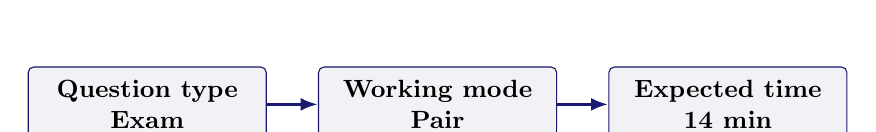
\begin{tikzpicture}[
node distance=0.65cm,
box/.style={draw=MidnightBlue, rounded corners=2pt, minimum height=0.95cm, align=center, font=\small\bfseries, fill=MidnightBlue!6, text width=0.23\linewidth},
arrow/.style={-{Latex[length=2.2mm]}, very thick, MidnightBlue}
]
\node[box] (type) {Question type\\Exam};
\node[box, right=of type] (mode) {Working mode\\Pair};
\node[box, right=of mode] (time) {Expected time\\14 min};
\draw[arrow] (type) -- (mode);
\draw[arrow] (mode) -- (time);
\end{tikzpicture}
\end{center}

{\large\bfseries\color{MidnightBlue} Prompt}\par\medskip
Using healthcare as your reference point, explain how the same hidden-state, noisy-evidence, belief-update, and action-choice pattern could also appear in autonomous driving, financial risk, or cybersecurity. Your answer should make clear what transfers and what stays domain-specific.

{\large\bfseries\color{MidnightBlue} Task details}\par\medskip
\begin{itemize}\item \textbf{Type:} exam
\item \textbf{Mode:} pair
\item \textbf{Time:} 14 min
\item \textbf{Deliverable:} structured synthesis response
\item \textbf{Assessment focus:} explain how the same uncertain-decision pattern transfers across domains
\item \textbf{Expected length:} 190-250 words\end{itemize}

{\large\bfseries\color{MidnightBlue} How to submit}\par\medskip
Post one pair Padlet comment comparing healthcare with one other domain and identifying what stays the same and what must change.

{\large\bfseries\color{MidnightBlue} Discussion in class}\par\medskip
Which part transfers well across domains, and which part stays domain-specific?

{\large\bfseries\color{MidnightBlue} Why this helps}\par\medskip
Supports capstone-style preparation through a fresh applied scenario.

{\large\bfseries\color{MidnightBlue} References}\par\medskip
\begin{itemize}\item Russell \& Norvig (2021) AIMA 4e, Ch.17-18
\item Poole \& Mackworth (2023) 3e, Ch.12-13, pp.517-608\end{itemize}
\end{tcolorbox}

\begin{tcolorbox}[colback=white,colframe=MidnightBlue,title={Q6 Stretch Extension},fonttitle=\bfseries,breakable]
\begin{center}
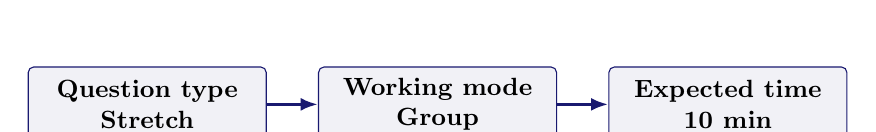
\begin{tikzpicture}[
node distance=0.65cm,
box/.style={draw=MidnightBlue, rounded corners=2pt, minimum height=0.95cm, align=center, font=\small\bfseries, fill=MidnightBlue!6, text width=0.23\linewidth},
arrow/.style={-{Latex[length=2.2mm]}, very thick, MidnightBlue}
]
\node[box] (type) {Question type\\Stretch};
\node[box, right=of type] (mode) {Working mode\\Group};
\node[box, right=of mode] (time) {Expected time\\10 min};
\draw[arrow] (type) -- (mode);
\draw[arrow] (mode) -- (time);
\end{tikzpicture}
\end{center}

{\large\bfseries\color{MidnightBlue} Prompt}\par\medskip
Define a compact monitoring dashboard for the healthcare capstone deployment. Cover four headings: clinical quality, operational load, safety, and trust. Give at least one metric for each heading.

{\large\bfseries\color{MidnightBlue} Task details}\par\medskip
\begin{itemize}\item \textbf{Type:} stretch
\item \textbf{Mode:} group
\item \textbf{Time:} 10 min
\item \textbf{Deliverable:} monitoring dashboard
\item \textbf{Assessment focus:} define a compact deployment dashboard for the capstone setting
\item \textbf{Expected length:} 4 categories + 1 metric each\end{itemize}

{\large\bfseries\color{MidnightBlue} How to submit}\par\medskip
Post one group Padlet comment with the four headings and one metric under each.

{\large\bfseries\color{MidnightBlue} Discussion in class}\par\medskip
Which single metric would you watch first during the first live week?

{\large\bfseries\color{MidnightBlue} Why this helps}\par\medskip
Good extension for evaluation, monitoring, and trustworthy deployment questions.

{\large\bfseries\color{MidnightBlue} References}\par\medskip
\begin{itemize}\item Russell \& Norvig (2021) AIMA 4e, Ch.17-18
\item Poole \& Mackworth (2023) 3e, Ch.12-13, pp.517-608\end{itemize}
\end{tcolorbox}

\section*{Submission Instructions}

Use the seeded Padlet posts for Q1--Q6. Q2 and Q3 are individual. Q1 and Q5 are pair tasks. Q4 and Q6 should be one joint group comment. Start each comment with your names or group label.

\section*{Whole-Class Debrief Prompts}

\begin{itemize}
\tightlist
\item
  Which of DBN, DDN, and POMDP plays the clearest role in the pipeline?
\item
  Where should the human gate sit in a high-risk workflow?
\item
  What changes most when you move the same pattern into another domain?
\end{itemize}

\section*{Exam Transfer Note (Day-Level)}

Maps to capstone exam preparation on DBN, DDN, POMDP, belief update, workflow design, and cross-domain transfer under uncertainty.

\end{document}
